%The principles behind designing for glass is to keep the information relevant. Google ranks different computational devices and services in terms of time periods. Google talks about how the cloud stores information ``forever'', a computer keeps about a years worth of information, a mobile phone is keeping track of the last month and Glass are for the present.\\

%Therefore Google asks developers to keep the information relevant and simple. Glass is designed not to get in the way of the user and, as stated previously, be usable when the users wants to.\cite{glassDesignPrinciples}\\
%\url{https://developers.google.com/glass/design/principles}

	\begin{figure}[ht!]
		\centering
		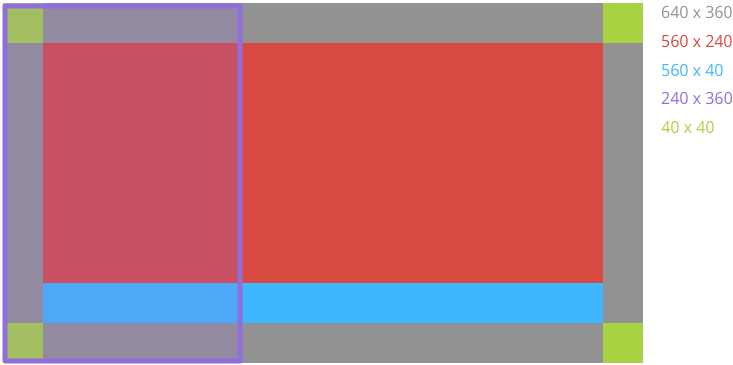
\includegraphics[width=110mm]{images/standard-template}
		\caption{Google provide developers with strict guidelines as to how they should use the limited space that Google Glass can present information on.\cite{glassDesignStyle}}
		\label{GlassDesignStyle}
	\end{figure}

%Google Glass is placed very close to the user's eye which makes the small projection seem Despite the fact that the display for Google Glass is placed very close to the user's eye the amount of information that can be displayed is still very limited. Google have therefore provided developers with a few guidelines when writing text which will be presented on Glass.\cite{glassDesignStyle} These guidelines, five in total,


% REWRITE !!!!
% \begin{itemize}
%	\item \textbf{Keep it brief.} Be concise, simple and precise. Look for alternatives to long text such as reading the content aloud, showing images or video, or removing features.
%	\item \textbf{Keep it simple.} Pretend you're speaking to someone who's smart and competent, but doesn't know technical jargon and may not speak English very well. Use short words, active verbs, and common nouns.
%	\item \textbf{Be friendly.} Use contractions. Talk directly to the reader using second person ("you"). If your text doesn't read the way you'd say it in casual conversation, it's probably not the way you should write it.
%	\item \textbf{Put the most important thing first.} The first two words (around 11 characters, including spaces) should include at least a taste of the most important information in the string. If they don't, start over. Describe only what's necessary, and no more. Don't try to explain subtle differences. They will be lost on most users.
%	\item \textbf{Avoid repetition.} If a significant term gets repeated within a screen or block of text, find a way to use it just once.
%\end{itemize}

%*** REWRITE !!!
